\documentclass[10pt, a4paper, italian]{article}
\usepackage[T1]{fontenc}
\usepackage[utf8]{inputenc}
\usepackage{amsmath, amssymb, amsthm, thmtools, amsfonts, mathtools}
\usepackage{nicefrac}
\usepackage{calc}
\usepackage[pdftex, hyperindex, plainpages=false]{hyperref}
\usepackage[nameinlink]{cleveref} %load before classicthesis (clash)
%\usepackage[nochapters,pdfspacing]{classicthesis}
\usepackage{siunitx}
\usepackage[siunitx]{circuitikz}

\usepackage[a4paper]{geometry}
\usepackage{float}
\usepackage{mdframed}
\usepackage{titling}
\usepackage{booktabs}
\usepackage{graphicx}
\usepackage{caption, subcaption}
\usepackage{xcolor}
\usepackage[italian]{babel}
\usepackage{pgfplots}
\usepackage{listings}
%\usepackage{lmodern}
\usepackage{url}
\usepackage{enumitem}
\usepackage{tikz} %loads after classicthesis (xcolor incompat)

% lets graphicx know path where figures to be included are found
\graphicspath{{../figs/}}
\makeatletter
\def\input@path{{../figs/}}
%or: \def\input@path{{/path/to/folder/}{/path/to/other/folder/}}
\makeatother

% tikz pgf plots setup
\usepgfplotslibrary{external}
\pgfplotsset{compat=1.15}
%\tikzexternalize

% spaces and significant digits/figures for measurements
\sisetup{free-standing-units, space-before-unit, number-unit-product = \;,
scientific-notation = false, round-mode = figures, round-precision = 1,}

% turns all (hyperlinked) references black [default is blue]
\hypersetup{
	linktoc=all,
	colorlinks=true,
	linkcolor=black
}

% code listings config
%\lstset{
%language=Python,
%basicstyle=\ttfamily,
%columns=fullflexible,
%keepspaces=true,
%}

% mdframed (for boxed text) configuration
\mdfsetup{linewidth=0.6pt}

% Default fixed font does not support bold face
\DeclareFixedFont{\ttb}{T1}{txtt}{bx}{n}{12} % for bold
\DeclareFixedFont{\ttm}{T1}{txtt}{m}{n}{12}  % for normal

% Custom colors
\usepackage{color}
\definecolor{deepblue}{rgb}{0,0,0.5}
\definecolor{deepred}{rgb}{0.6,0,0}
\definecolor{deepgreen}{rgb}{0,0.5,0}

% Commands 
\newcommand{\executeiffilenewer}[3]{%
	\ifnum\pdfstrcmp{\pdffilemoddate{#1}}%
		{\pdffilemoddate{#2}}>0%
	{\immediate\write18{#3}}\fi%
}
% input .svg --> .pdf_tex graphs
%\newcommand{\includesvg}[1]{%
%	\executeiffilenewer{#1.svg}{#1.pdf}%
%	{inkscape -z -D --file=#1.svg %
%	--export-pdf=#1.pdf --export-latex}%
%	\input{#1.pdf_tex}%
%}
% Thanks UniPi's Department of Physics E. Fermi
\newcommand{\thanksdf}{(\thanks{Dipartimento di Fisica E.~Fermi,%
Universit\`a di Pisa - Pisa, Italy.}\;)}

% hyperlink to email address
\newcommand{\mail}[1]{\href{mailto:#1}{\textsf{#1}}}

% \vec for bold vectors, instead of overarrows (now "\arrvec")
\let\arrvec=\vec
\renewcommand{\vec}[1]{\boldsymbol #1}
% replaces straight phi with slanted phi
\renewcommand{\phi}{\varphi}
% replaces straight eps with curved epsilon
\newcommand{\eps}{\varepsilon}
% abbreviation for (sub_/super^)scripts of \lim, \sum,... in inline math
\newcommand{\ds}{\displaystyle}

% blackboard/number set letters
\newcommand{\CC}{\mathbb C}
\newcommand{\HH}{\mathbb H}
\newcommand{\KK}{\mathbb K}
\newcommand{\NN}{\mathbb N}
\newcommand{\PP}{\mathbb P}
\newcommand{\QQ}{\mathbb Q}
\newcommand{\RR}{\mathbb R}
\newcommand{\ZZ}{\mathbb Z}

\newcommand{\Abs}[1]{{\left\Vert #1\right\Vert}}
\newcommand{\enclose}[1]{{\left( #1 \right)}}
\newcommand{\Enclose}[1]{{\left[ #1 \right]}}
\newcommand{\floor}[1]{\left\lfloor #1 \right\rfloor}
\newcommand{\ceil}[1]{\left\lceil #1 \right\rceil}
\newcommand{\To}{\rightrightarrows}

% Math operators
\DeclareMathOperator{\divergence}{div}
\renewcommand{\div}{\divergence}
\DeclareMathOperator{\Imaginarypart}{Im}
\renewcommand{\Im}{\Imaginarypart}
\DeclareMathOperator{\Realpart}{Re}
\renewcommand{\Re}{\Realpart}
%\DeclareMathOperator{\arg}{arg}
\DeclareMathOperator{\tg}{tg}
\DeclareMathOperator{\arctg}{arctg}
\DeclareMathOperator{\settsinh}{settsinh}
\DeclareMathOperator{\settcosh}{settcosh}
\DeclareMathOperator{\tr}{tr}
\DeclareMathOperator{\im}{im}
\DeclareMathOperator{\sgn}{sgn}
\DeclareMathOperator{\diag}{diag}

\DeclarePairedDelimiter{\norm}{\lVert}{\rVert}
\DeclarePairedDelimiter{\scalar}{\langle}{\rangle}

% Logarithm with arbitrary base.
% -> log_10
\newcommand{\llog}[1][10]{\log_{#1}}

% Absolute value.
% -> |x|
\newcommand{\abs}[1]{\left| #1 \right|}

% Powers.
% -> x^a
\newcommand{\power}[2][2]{\left( #2 \right)^{#1}}

% Square.
% -> x^2
\newcommand{\sq}[1]{\power[2]{#1}}

% Expansion of the binomial coefficient.
% -> n1!/(n2!(n1 - n2)!)
\newcommand{\binomexpr}[2]{\frac{#1!}{#2!(#1 - #2)!}}

% Expression evaluation at a given point with square brackets.
% -> [x]_{a}
\newcommand{\at}[2]{\left[ #1\right]_{\makebox[-1pt][l]{${\scriptstyle#2}$}}}

% Expression evaluation in an interval.
% -> [x] _{a}^{b}
\newcommand{\eval}[3]{\left.#1%
  \right|_{\makebox[-1pt][l]{${\scriptstyle#2}$}}^{\makebox[-1pt][l]{${\scriptstyle#3}$}}}

% Upright d in math mode (for differentials).
% -> d
\newcommand{\ud}{\mathrm{d}}

% Differential.
% -> dx
\newcommand{\diff}[1][x]{\,\ud{#1}}

% Base command for defining derivatives.
% -> df/dx or d^kf/dx^k
\newcommand{\basederivative}[4][]{%
  \displaystyle%
  \ifx\\#1\\\frac{#4#2}{#4#3}%
  \else%
  \frac{#4^#1#2}{#4#3^#1}%
  \fi%
}

% Total derivative.
% -> df/dx(x) or d^kf/dx^k(x)
\newcommand{\td}[4][]{%
  \basederivative[#1]{#2}{#3}{\ud}%
  \ifx\\#4\\%
  \else%
  \mkern-4mu\left(#4\right)%
  \fi%
}

% Partial derivative.
% -> df/dx(x) or d^kf/dx^k(x)
\newcommand{\pd}[4][]{%
  \basederivative[#1]{#2}{#3}{\partial}%
  \ifx\\#4\\%
  \else%
  \mkern-4mu\left(#4\right)%
  \fi%
}

\newcommand{\intinf}{\int_{-\infty}^{\infty}\!\!\!}

\newcommand{\cinterval}[2]{\left[\, #1,~#2 \,\right]}

\newcommand{\linterval}[2]{\left[\, #1,~#2 \,\right)}

\newcommand{\rinterval}[2]{\left(\, #1,~#2 \,\right]}

\newcommand{\ointerval}[2]{\left(\, #1,~#2 \,\right)}

\newcommand{\prob}[1]{\displaystyle P\left(#1\right)}

\newcommand{\pvalue}{\emph{$p$-value}}

\newcommand{\cond}{\,|\,}

\newcommand{\expect}[1]{\displaystyle E\left[#1\right]}

\newcommand{\mom}[2][]{\displaystyle {\cal M}_{#2}\ifx\\#1\\\else(#1)\fi}

\newcommand{\momalg}[1]{\displaystyle \lambda_{#1}}

\newcommand{\momcen}[1]{\displaystyle \mu_{#1}}

\newcommand{\skewness}{\displaystyle \gamma_1}

\newcommand{\kurtosis}{\displaystyle \gamma_2}

\newcommand{\charf}[1][x]{\phi_{#1}}

\newcommand{\momgenf}[1][x]{M_{#1}}

\newcommand{\fwhm}{{\scriptstyle \textsc{FWHM}}}

\newcommand{\hwhm}{{\scriptstyle \textsc{HWHM}}}

\newcommand{\median}{\mu_{\nicefrac{1}{2}}}

\newcommand{\var}[1]{\ensuremath{\text{Var}\left(#1\right)}}

\newcommand{\cov}[2]{\ensuremath{\text{Cov}\left(#1, #2\right)}}

\newcommand{\corr}[2]{\ensuremath{\text{Corr}\left(#1, #2\right)}}

\newcommand{\like}{\mathcal L}

\newcommand{\likelihood}[2][]{\like\ifx\\#2\\\else(#2\ifx\\#1\\\else;#1\fi)\fi}

\newcommand{\chisq}{\ensuremath{\chi^2}}

\newcommand{\chisquare}[2][]{\chisq\ifx\\#2\\\else(#2\ifx\\#1\\\else;#1\fi)\fi}

\newcommand{\loglikelihood}[2][]{\log\likelihood[#1]{#2}}

\newcommand{\pdf}[3][]{#2(#3\ifx\\#1\\\else;#1\fi)}

\newcommand{\binomialpdf}[2][]{\pdf[#1]{\mathcal B}{#2}}

\newcommand{\multinomialpdf}[2][]{\pdf[#1]{\mathcal M}{#2}}

\newcommand{\poissonpdf}[2][]{\pdf[#1]{\mathcal P}{#2}}

\newcommand{\uniformpdf}[2][]{\pdf[#1]{u}{#2}}

\newcommand{\exponentialpdf}[2][]{\pdf[#1]{\varepsilon}{#2}}

\newcommand{\gausspdf}[2][]{\pdf[#1]{N}{#2}}

\newcommand{\chisquarepdf}[2][]{\pdf[#1]{\wp}{#2}}

\newcommand{\cauchypdf}[2][]{\pdf[#1]{c}{#2}}

\newcommand{\erf}[1]{\ensuremath{\text{erf}\left(#1\right)}}

\newcommand{\dccases}[4][]{#2 \ifx\\#2\\\else=\fi %
  \begin{cases}
    \displaystyle #3 & \text{per variabili discrete}\\
    \displaystyle #4 & \text{per variabili continue}#1
  \end{cases}
}
% sub/super-scriptable for all symbol as math operator 
\newcommand\Scaleforall[1]{\vcenter{\hbox{\scalefont{#1}$\forall$}}}

\DeclareMathOperator*\forevery{%
  \vphantom\sum
  \mathchoice{\Scaleforall{2}}{\Scaleforall{1.4}}{\Scaleforall{1}}{\Scaleforall{0.75}}}
\usepackage{multicol}
\usepackage{placeins}
\usepackage{diagbox}
\geometry{left=2cm, right=2cm, top=2cm, bottom=2cm}

% indexes subsections with letters, sections with numbers (1.a, 1.b, ...)
\renewcommand{\thesubsection}{\thesection.\alph{subsection}}

% lets graphicx know path where figures to be included are found
\graphicspath{{../figs/}}

\author{Gruppo 1.AC \\ Matteo Rossi, Bernardo Tomelleri}
\title{EsD1: Caratterizzazione di porte logiche e semplici circuiti logici.}
\begin{document}
\date{\today}
\maketitle

\setcounter{section}{0}

\section{Misura componenti dei circuiti}
\begin{table}[htbp]
\centering
\begin{tabular}{ccc}
\toprule
Resistenze $[\si{\ohm}]$ & $R$ & $\sigma R$ \\
\midrule
\midrule
$R\ped{pot}$	& 9.53 k	& 0.08 k 		\\
$R_0$	  		& 993		& 8				\\
$R_1$	  		& 992		& 8	 			\\
$R_2$	  		& 993		& 8	 			\\
$R_3$	  		& 994		& 8	 			\\
$R_4$	  		& 997		& 8	 			\\
\bottomrule     
\end{tabular}
\caption{Valori di resistenza misurati per i componenti passivi dei circuiti
studiati. \label{tab: rmesB}}
\end{table}

\begin{table}[htbp]
\centering
\begin{tabular}{ccc}
\toprule
Resistenze $[\si{\ohm}]$ & $R$ & $\sigma R$ \\
\midrule
\midrule
$R\ped{pot}$	& 9.53 k	& 0.08 k 		\\
$R_0$	  		& 993		& 8				\\
$R_1$	  		& 992		& 8	 			\\
$R_2$	  		& 993		& 8	 			\\
$R_3$	  		& 994		& 8	 			\\
$R_4$	  		& 997		& 8	 			\\
\bottomrule     
\end{tabular}
\caption{Valori di resistenza misurati per i componenti passivi dei circuiti
studiati. \label{tab: rmesB}}
\end{table}

Riportiamo per completezza anche il valore della tensione continua di
alimentazione continue per i circuiti integrati misurata con il multimetro
\begin{align*}
V_{CC} &= 4.99 \pm 0.03 \si{\V} \\
\end{align*}

\subsection*{Nota sul metodo di fit}
Per determinare i parametri ottimali e le rispettive covarianze si \`e
implementato in \verb+Python+ un algoritmo di fit basato sui minimi quadrati
mediante la funzione \emph{curve\_fit} della libreria \texttt{SciPy}.

%=======================
\section{Caratteristiche fisiche delle porte logiche}
\begin{minipage}{0.7\textwidth}
    Il punto di questa sezione è quello di verificare che l'integrato preso in esame, SN7404 a porte NOT (raffigurato a fianco), rientri nelle specifiche del DS. Per fare questo ci focalizziamo su alcune grandezze che descrivono il nostro integrato e che espliciteremo in dettaglio di seguito. In questa prima parte ci focalizzeremo più su un'analisi qualitativa.\\
    Per le nostre misure, alimentiamo il TTL con una ddp di 5 V.
\end{minipage}
\begin{minipage}{0.3\textwidth}
    %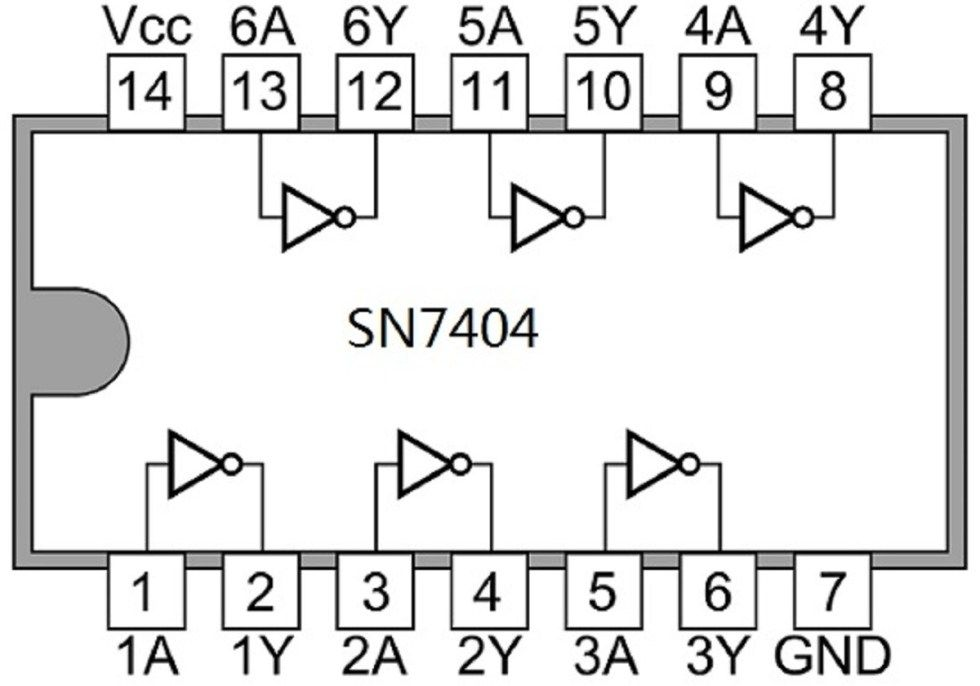
\includegraphics[width=\textwidth]{NOT.png}
    \label{NOT}
\end{minipage}

\subsection{Tensioni di operazione}
Come prime misure verifichiamo i valori delle tensioni di soglia in ingresso e tipiche in uscita, da cui è possibile ricavare il Noise Margin.\\
%la definizione di noise margin prevede di usare i valori minimi e massimi ma nella scheda chiede di trovare le tensioni tipiche: infatti anche sul datasheet sono riportate sia quelle min e max che quelle typ per i valori in output.. magari vediamo che valori ci escono
Generiamo una rampa di tensione 0-5 V e visualizziamo i segnali prodotti:
in questo modo è possibile costruire un grafico di $V_{out}$ in funzione di $V_{in}$.\\ %possiamo usare sia dalla modalità XY che prendendo i dati, magari possiamo fare entrambe le cose e vedere qual è meglio..
Possiamo quindi misurare i valori del Noise Margin High e Low definiti rispettivamente
\begin{gather*}
    NM_H=V_{OH,min}-V_{IH,min}\\
    NM_L=V_{IL,max}-V_{OL,max}
\end{gather*}
Dove $V_{OH,min}$ è il minimo valore interpretato in output dalla porta come alto; analogamente possiamo descrivere le altre grandezze presenti nelle definizioni.\\
Dalle specifiche del DS si ha che i valori attesi sono %non ho visto gli errori
\begin{multicols}{2}
    \centering
    $V_{OH,min}=$ 2.4 V\\ %typ 3.4 V
    $V_{IH,min}=$ 2 V\\
    $NM_H=$ 0.4 V
    
    $V_{IL,max}=$ 0.8 V\\
    $V_{OL,max}=$ 0.4 V\\ %typ 0.2 V
    $NM_L=$ 0.4 V
\end{multicols}
Dalle nostre misure otteniamo %spiegare come abbiamo misurato
\begin{multicols}{2}
    \centering
    $V_{OH,min}=$ $\pm$ V\\
    $V_{IH,min}=$ $\pm$ V\\
    $NM_H=$ $\pm$ V
    
    $V_{IL,max}=$ $\pm$ V\\
    $V_{OL,max}=$ $\pm$ V\\
    $NM_L=$ $\pm$ V
\end{multicols}
(dire se torna)

\subsection{Misura del Fan-out}
Il Fan-out è il numero massimo di porte che una singola porta può guidare restando entro le specifiche di funzionamento ed è definito nel seguente modo
\[
\mbox{Fan-out}=\frac{I_{OH,max}}{I_{IH,max}}
\]
Dalle specifiche del DS leggiamo
\begin{gather*}
    I_{IH,max}=-0.4 mA\\
    I_{OH,max}= 40 \mu A\\
    \mbox{Fan-out}=-0.1 (?) %Probabilmente vanno presi i valori assoluti però non mi torna molto che sia minore di uno...
\end{gather*}
Misuriamo le correnti\\ %non so se vogliamo descrivere un minimo il procedimento come sulla scheda..
input a 2.4V ale 12 uA eli  13uA ele 21uA
output a 3.4V ale 1.21 mA eli 1.13 ele 1.54mA
(output 2 ?? ele 0.375 mA)
\section{Circuiti logici elementari}
\begin{minipage}{0.65\textwidth}
    In questa sezione, dopo aver rimosso l'integrato analizzato nella sezione precedente, utilizziamo due integrati del tipo SN74LS00 a porte NAND a due ingressi, schematizzati nella figura a lato. Una fondamentale caratteristica delle porte NAND è la loro universalità, ossia il fatto che è possibile realizzare qualsiasi tipo di circuito: infatti, con combinazioni di porte NAND, possiamo ottenere circuiti equivalenti dalle porte AND, OR e NOT, a partire dalle quali è possibile realizzare qualsiasi circuito.
\end{minipage}
\begin{minipage}{0.35\textwidth}
    %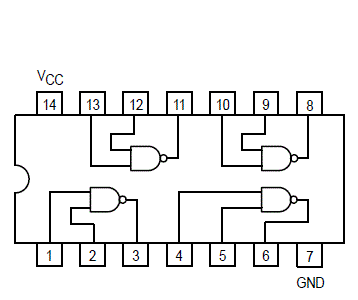
\includegraphics[width=\textwidth]{NAND.png}
    \label{NAND}
\end{minipage}

\subsection{Tabella di verità}
Dalla funzione StaticIO visualizziamo la tabella di verità e la verifichiamo utilizzando gli interruttori.\\
\\
(Utilizzando le funzioni Pattern di Waveform producete le quattro possibili coppie di valori in ingresso e con la funzione Logic acquisite questi due segnali assieme al segnale in uscita e riportate il grafico nella relazione)\\
\\
Producendo, tramite la funzione Pattern, le quattro coppie degli ingressi, riportiamo le acquisizioni dei segnali visualizzati con Logic.\\
\\
Riportiamo inoltre il grafico (che grafico?)

\subsection{Circuiti con porte NAND}
In questa sezione vogliamo analizzare dei circuiti con il solo utilizzo di porte NAND.\\
\\
(Riportare per ognuno:\\
la derivazione analitica, utilizzando l'algebra di Boole, che trasformi la funzione logica desiderata in soli NAND;\\
lo schema del circuito;\\
un'acquisizione effettuata utilizzando le funzioni Pattern e Logic che dimostri la funzionalità del circuito.)

\subsubsection*{Circuito 1}
Come primo circuito vogliamo realizzare una porta OR: detti \textit{A} e \textit{B} gli ingressi e \textit{Y} l'uscita, nella notazione dell'algebra booleana si ha
\[
    Y=A+B
\]
Sfruttando la legge di De Morgan si ottiene
\[
    Y=A+B=\overline{\overline{A}\cdot\overline{B}}
\]
che descrive la relazione OR in termini del NAND.\\
Nota la relazione per ottenere un NOT utilizzando porte NAND, riportiamo lo schema del circuito
\begin{figure}[htb!]
    \centering
    %\includegraphics[width=0.45\textwidth]{OR.png}
    \label{or}
\end{figure}
\FloatBarrier

\subsubsection*{Circuito 2}
Realizziamo un circuito che permetta di assegnare all'uscita il valore di uno dei due ingressi a singolo bit tramite il valore di un terzo ingresso.
Indichiamo con \textit{A}, \textit{B} e \textit{C} gli ingressi e con \textit{Y} l'uscita; il funzionamento del nostro circuito può essere descritto dalla tabella di Karnaugh riportata sotto\\
\begin{minipage}{0.5\textwidth}
    \[
    \begin{cases}
    C=0 \implies Y=A\\
    C=1 \implies Y=B
    \end{cases}
    \]
\end{minipage}
\begin{minipage}{0.3\textwidth}
    \centering
    \begin{tabular}{c||c|c|c|c}
        \backslashbox{C}{AB} & 00 & 01 & 11 & 10\\
        \hline
        \hline
        0 & 0 & 0 & 1 & 1\\
        \hline
        1 & 0 & 1 & 1 & 0\\
    \end{tabular}
\end{minipage}
\newline
\newline
da cui si ricava facilmente la seguente relazione per il circuito
\[
Y=A\cdot\overline{C}+B\cdot C
\]
e, sempre sfruttando De Morgan, si ha
\[
Y=A\cdot\overline{C}+B\cdot C=\overline{(\overline{A\cdot\overline{C}})\cdot(\overline{B\cdot C})}
\]
Riportiamo sotto lo schema del circuito
\begin{figure}[htb!]
    \centering
    %\includegraphics[width=0.6\textwidth]{cir2.png}
    \label{circuito2}
\end{figure}
\FloatBarrier
Per dimostrare il corretto funzionamento del circuito riportiamo le acquisizioni di Pattern, in cui è possibile comprendere come sono stati impostati gli ingressi, e Logic, da cui si può verificare il corretto funzionamento del circuito.
\begin{figure}[htb!]
    \centering
    %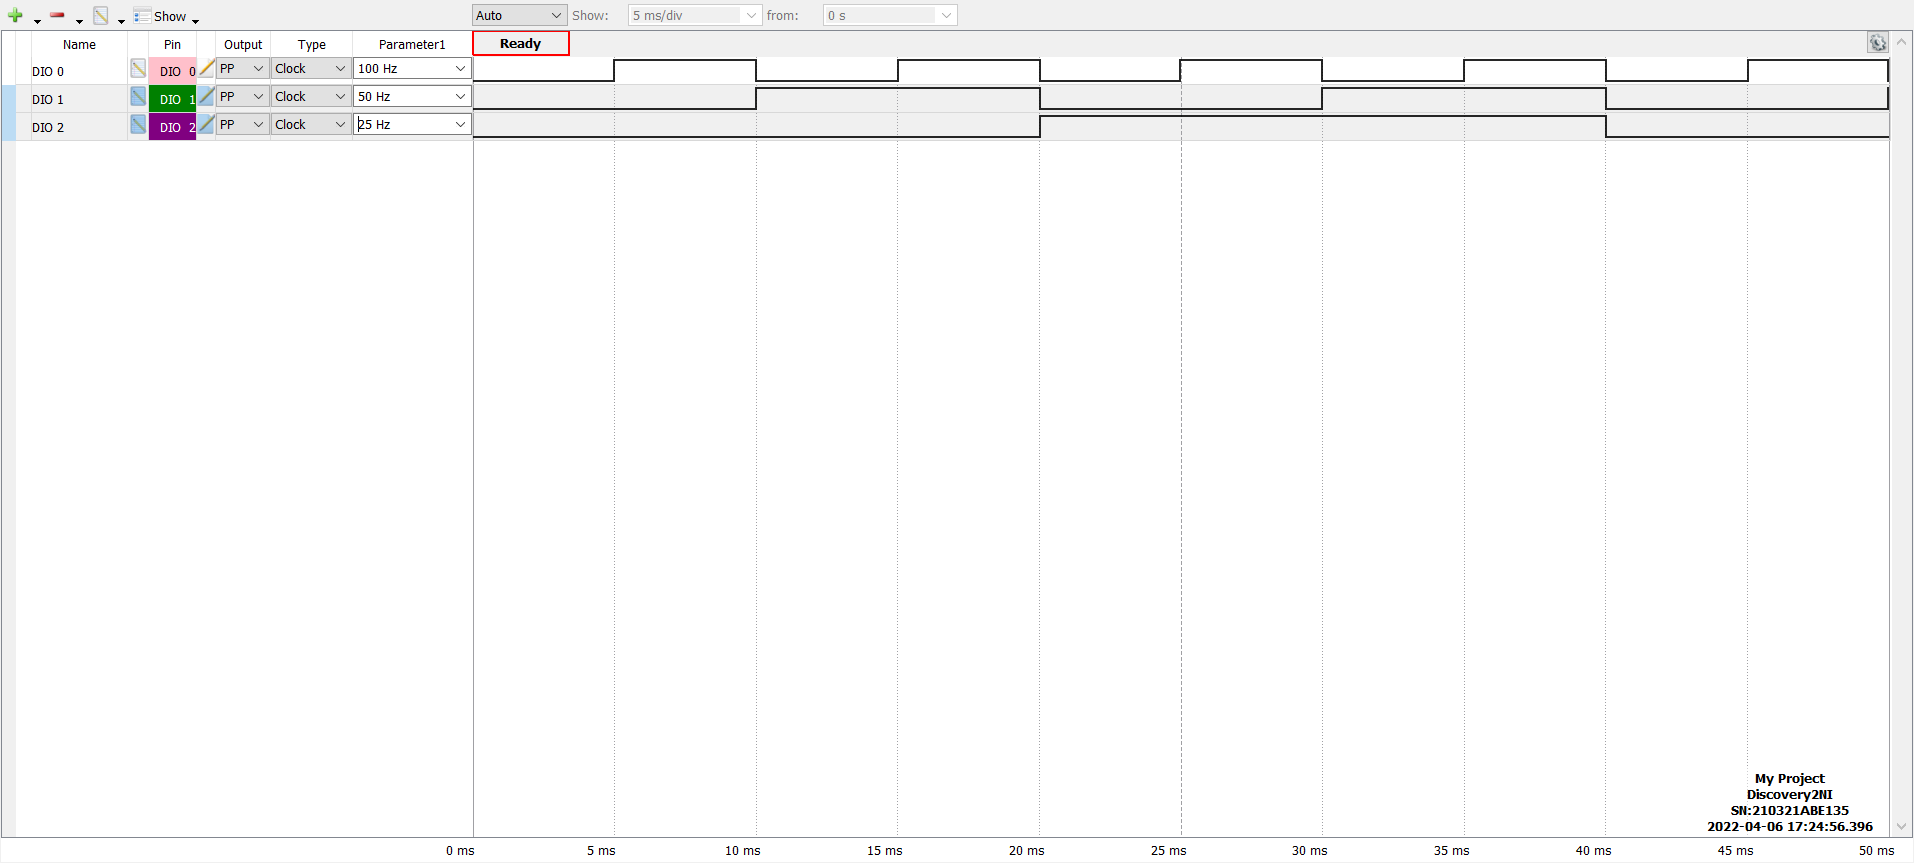
\includegraphics[width=0.8\textwidth]{pat2.png}
    \caption{Pattern: DIO 0 $\equiv$ C, DIO 1 $\equiv$ A e DIO 2 $\equiv$ B}
    \label{pat2}
\end{figure}
\FloatBarrier
\begin{figure}[htb!]
    \centering
    %\includegraphics[width=0.8\textwidth]{log2.png}
    \caption{Logic: DIO 0 $\equiv$ C, DIO 1 $\equiv$ A, DIO 2 $\equiv$ B e DIO 3 $\equiv$ Y}
\end{figure}
\FloatBarrier

\section{Convertitore Gray-Binario}
\begin{minipage}{0.7\textwidth}
    Come ultima cosa vogliamo realizzare un circuito in grado di convertire un valore a 4 bit dalla codifica Gray in Binario utilizzando un solo integrato di tipo SN74LS86 a porte XOR, descritto nella figura a lato.\\
    Un convertitore Gray-Binario può essere schematizzato come in Figura (\ref{gb}): il nostro obiettivo è quello di verificare che tale circuito si comporti come atteso.
\end{minipage}
\begin{minipage}{0.3\textwidth}
    %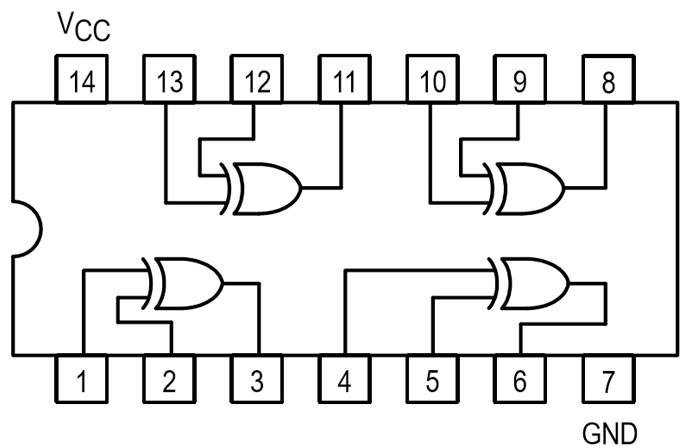
\includegraphics[width=\textwidth]{XOR.png}
\end{minipage}
\newline
\begin{minipage}{0.5\textwidth}
    \centering
    %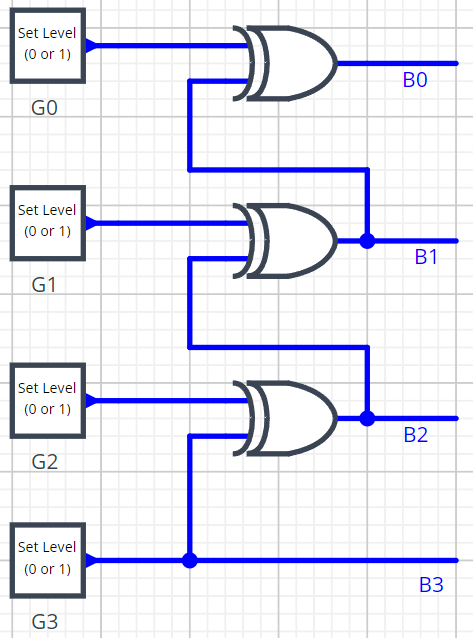
\includegraphics[width=0.8\textwidth]{gb.png}
    \captionof{figure}{Schema convertitore Gray-Binario}
    \label{gb}
\end{minipage}
\begin{minipage}{0.5\textwidth}
    \centering
    \begin{tabular}{c||c}
        Codice binario & Codice Gray \\
        \hline
        \hline
        0000 & 0000\\
        0001 & 0001\\
        0010 & 0011\\
        0011 & 0010\\
        0100 & 0110\\
        0101 & 0111\\
        0110 & 0101\\
        0111 & 0100\\
        1000 & 1100\\
        1001 & 1101\\
        1010 & 1111\\
        1011 & 1110\\
        1100 & 1010\\
        1101 & 1011\\
        1110 & 1001\\
        1111 & 1000\\
        \end{tabular}
    \captionof{table}{Conteggio a 4 bit nei due codici.}
    \label{grbin}
\end{minipage}
\newline
\newline
Il codice Gray differisce dal codice binario in quanto si passa da un intero al successivo modificando un solo bit per volta.\\
Calcoliamo l'uscita del circuito per alcuni valori in ingresso:
\begin{table}[htb!]
    \centering
    \[
    \begin{array}{cccc|cccc}
        G_3 & G_2 & G_1 & G_0 & B_3 & B_2 & B_1 & B_0\\
        \hline
        0 & 0 & 0 & 0 & 0 & 0 & 0 & 0\\
        1 & 1 & 1 & 1 & 1 & 0 & 1 & 0\\
        1 & 0 & 0 & 1 & 1 & 1 & 1 & 0\\
        1 & 0 & 0 & 0 & 1 & 1 & 1 & 1\\
    \end{array}
    \]
\end{table}
\FloatBarrier
Confrontando le uscite ottenute con i valori riportati in Tabella (\ref{grbin}) affermiamo che il circuito si comporta correttamente come convertitore Gray-Binario. Come conferma, riportiamo un'acquisizione.\\
\begin{figure}[htb!]
    \centering
    %\includegraphics[width=\textwidth]{figs:gray/gray.png}
    \caption{Acquisizione del Logic Analyzer per un ciclo completo (frequenza 10 Hz) dei segnali in ingresso e in uscita dal convertitore Gray-binario.}
\end{figure}
\begin{figure}[htb!]
    \centering
    %\includegraphics[width=\textwidth]{figs:gray/gray_transition_30ns.png}
    \caption{Acquisizione del Logic Analyzer durante la transizione dal numero $15$ al numero $0$ su scala dei tempi pari a $30$ ns. Il primo cursore evidenzia la durata di una metà del glitch su DIO 9 ($10$ ns) mentre il secondo è posto a $60$ ns per individuare la durata complessiva del glitch in DIO 11.}
\end{figure}
Per una scala dei tempi molto stretta, si registra che i tempi di propagazione non sono istantanei, distinguendo dei glitch(s) sui canali di uscita. \\
In particolare, per DIO 9 (B1 

\begin{figure}[htb!]
    \centering
    %\includegraphics[width=\textwidth]{figs:gray/gray_transition_10ns.png}
    \caption{Transizione dal $15$ allo $0$ su scala temporale pari a $10$ ns. Si riporta la tendina degli Eventi rilevanti per il canale DIO 11 (output B3: MSB).}
\end{figure}
(verificate il funzionamento del circuito utilizzando Pattern per generare un contatore a 4 bit con la codifica opportuna e osservando l’uscita con Logic (come ai punti precedenti);\\
osservate su una scala molto stretta (30ns) la transizione dal numero 15 al numero 0;\\
motivate l’osservazione del punto precedente tenendo conto del tempo di propagazione necessario per i due circuiti;\\
riportate tutti i grafici necessari a dimostrare il funzionamento del circuito.)

\subsection{Sommatore a 2 bit}
Vogliamo costruire un sommatore a due bit utilizzando le dovute porte logiche. Utilizzeremo i chip \texttt{SN74LS08} (quad-AND), \texttt{SN74LS32} (quad-OR), \texttt{SN74LS86} (quad-XOR). Il circuito da montare è riportato in Fig.(\ref{fig:fulladder}).

\begin{figure}[htbp]
    \centering
%    \includegraphics[width=0.6\linewidth]{fulladder.png}
    \caption{Schema circuitale di un sommatore a due bit.}
    \label{fig:fulladder}
\end{figure}

Verifichiamo il funzionamento mandando in ingresso tutte le possibili combinazioni di due numeri a due bit. Per fare ciò mandiamo ai 4 ingressi del circuito un segnale che conta in binario. Il risultato è mostrato in Fig.(\ref{fig:faAD2}).

\begin{figure}[htbp]
    \centering
%    \includegraphics[width=\linewidth]{fulladderAD2.png}
    \caption{Andamento del sommatore, si consulti la colonna di sinistra per il significato di ciascuna riga.}
    \label{fig:faAD2}
\end{figure}

Aggiungiamo al circuito 4 led verdi e un led rosso: questi sono pilotati da 5 nuovi cavi dell'AD2. Per controllare il loro funzionamento aggiungiamo a \emph{Patterns} una tabella delle verità, riportata in \ref{fig:Ver}, che faccia in modo che ad ogni step si illuminino un numero di led pari al valore della somma. Il led rosso verrà usato per controllare l'overflow, ovvero la possibilità che il risultato sia maggiore o uguale a 5. Per osservare al meglio il risultato si può vedere il video registrato per l'occasione, reperibile al link seguente: \url{https://www.youtube.com/watch?v=D473oqeD6gc}.

\begin{figure}[htbp]
    \centering
%    \includegraphics[width=0.8\linewidth]{ROM.PNG}
    \caption{Tabella delle verità usata.}
    \label{fig:Ver}
\end{figure}

%=======================
\section*{Conclusioni e commenti finali}
Si è riusciti a costruire e caratterizzare un amplificatore di tensione
invertente con un JFET in configurazione a emettitore comune. In particolare
si è riusciti ad apprezzare il differente comportamento (anche non lineare)
del circuito in vari regimi, dare una stima di guadagno, impedenza in
ingresso e frequenze caratteristiche della sua risposta in frequenza.

%=======================
\section*{Dichiarazione}
I firmatari di questa relazione dichiarano che il contenuto della relazione \`e
originale, con misure effettuate dai membri del gruppo, e che tutti i firmatari
hanno contribuito alla elaborazione della relazione stessa.

\end{document}
